%
% Copyright (C) 2004-2009 Jason Blevins <jrblevin@sdf.lonestar.org>
% http://jblevins.org/projects/cv-template/
%
% You may use use this document as a template to create your own CV
% and you may redistribute the source code freely. No attribution is
% required in any resulting documents. I do ask that you please leave
% this notice and the above URL in the source code if you choose to
% redistribute this file.

\documentclass[letterpaper, 11pt]{article}

\usepackage{hyperref}
\usepackage{geometry}

%%%%%%%%%%%%%%%%%%%%%%%%%%%%%%%%%%%%%%%%%%%%%%%%%%%%%%%%%%%%%%%%%%%%%%%%%%%%%%%%%
\usepackage[minbibnames=3,sorting=ndymdt,date=comp,isbn=false,doi=false,defernumbers=true,backend=biber]{biblatex}
\addbibresource[]{papers.bib}
\addbibresource[]{presentations-conference.bib}
\addbibresource[]{presentations-invited.bib}
\addbibresource[]{presentations-other.bib}

\DeclareSortingTemplate{ndymdt}{
	\sort[direction=descending]{
		\field{sortyear}
		\field{year}
		\literal{9999}
	}
	\sort[direction=descending]{
		\field[padside=left,padwidth=2,padchar=0]{month}
		\literal{99}
	}
	\sort[direction=descending]{
		\field[padside=left,padwidth=2,padchar=0]{day}
		\literal{99}
	}
	\sort{
		\field{presort}
	}
	\sort[final]{
		\field{sortkey}
	}
	\sort{
		\field{sortname}
		\field{author}
		\field{editor}
		\field{translator}
		\field{sorttitle}
		\field{title}
	}
	\sort{
		\field{sorttitle}
	}
	\sort[direction=descending]{
		\field[padside=left,padwidth=4,padchar=0]{volume}
		\literal{9999}
	}
}

\usepackage{graphicx}



%\usepackage[sfdefault]{cabin}
%\usepackage[T1]{fontenc}

%\usepackage[sfdefault]{overlock} %% Option 'sfdefault' only if the base font of the document is to be sans serif
\usepackage[default,oldstyle,scale=0.95]{opensans}

\usepackage[T1]{fontenc}

\usepackage{enumitem}
\usepackage{setspace}
	\onehalfspacing
\usepackage{xcolor}

% Set your name here
\def\name{George G. Vega Yon}

% Replace this with a link to your CV if you like, or set it empty
% (as in \def\footerlink{}) to remove the link in the footer:
\def\footerlink{https://ggvy.cl}

% The following metadata will show up in the PDF properties
\hypersetup{
  colorlinks = true,
  urlcolor = teal,
  pdfauthor = {\name},
  pdfkeywords = {economics, statistics, mathematics},
  pdftitle = {\name: Curriculum Vitae},
  pdfsubject = {Curriculum Vitae},
  pdfpagemode = UseNone
}

\geometry{
%  body={6.5in, 9in},
  left=1in,
  top=1in,
  right=1in,
  bottom=1in
}

% Customize page headers
\usepackage{fancyhdr}
%\pagestyle{myheadings}
%\markright{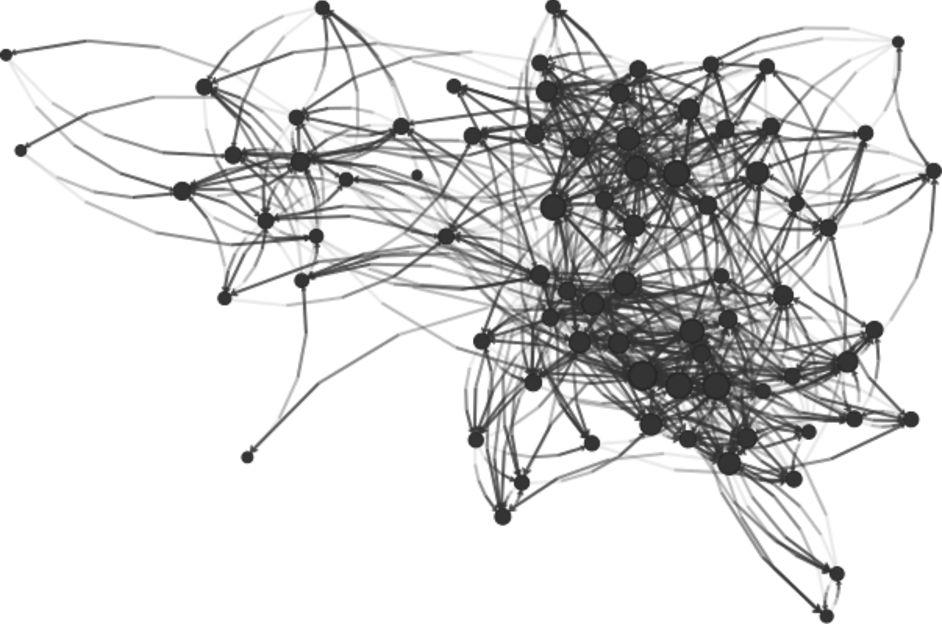
\includegraphics[width=1cm]{fig/ukfaculty.pdf} \name}
\pagestyle{fancy}
\fancyhead{}
\fancyfoot{}
\renewcommand{\headrulewidth}{0pt}
\fancyhead[L]{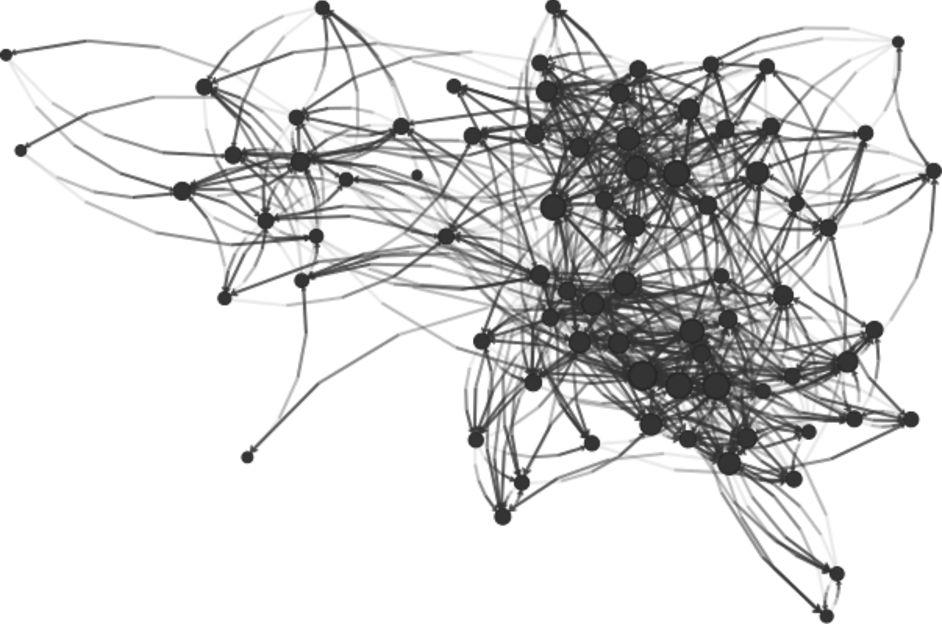
\includegraphics[width=1cm]{fig/ukfaculty.pdf}\\\vspace{-.75cm}\hspace{1.1cm}\emph{\name}}
\fancyhead[R]{\small\thepage}
\thispagestyle{empty}

% Custom section fonts
%\usepackage{sectsty}
%\sectionfont{\sffamily\mdseries\Large}
%\subsectionfont{\sffamily\mdseries\itshape\large}

% Other possible font commands include:
% rmfamily
% \ttfamily for teletype,
% \sffamily for sans serif,
% \bfseries for bold,
% \scshape for small caps,
% \normalsize, \large, \Large, \LARGE sizes.

% Don't indent paragraphs.
\setlength\parindent{0em}

% Make lists without bullets
%\renewenvironment{itemize}{
%  \begin{list}{}{
%    \setlength{\leftmargin}{0.45cm}
%  }
%}{
%  \end{list}
%}

% Para poder poner comandos genericos en tablas (en el inicio del argumento)
\usepackage{array}

\renewcommand{\bf}{\bfseries\color{teal}}
\renewcommand{\textbf}[1]{{\bfseries\color{teal}#1}}

\begin{document}

% Place name at left
\hfill 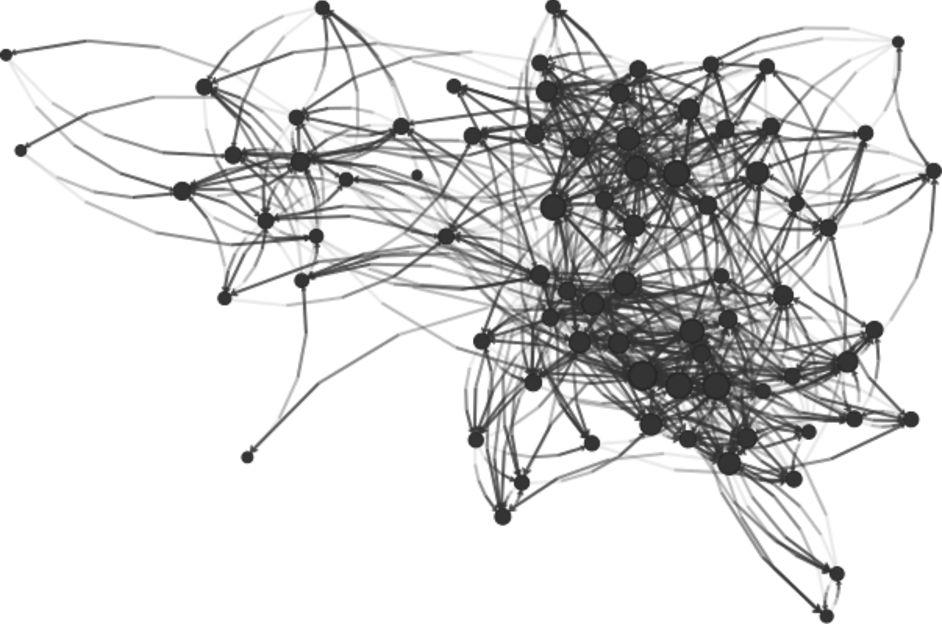
\includegraphics[width=.4\linewidth]{fig/ukfaculty.pdf}\vspace{-6cm}
\part*{\color{darkgray}{\name}}
% Alternatively, print name centered and bold:
%\centerline{\huge \bf \name}

%\vspace{0.25in}

\begin{minipage}{0.50\linewidth}
  \begin{tabular}{>{}p{.2\linewidth}p{.79\linewidth}}
    Mobile & +1 (six two six) 381 8171 \\
    e-mail & \href{mailto:g.vegayon@gmail.com}{\tt g.vegayon@gmail.com} \\
    website & \href{https://ggvy.cl}{\tt ggvy.cl} \\
    Code & \href{https://github.com/gvegayon}{\tt github.com/gvegayon}\\
    Linkedin & \href{https://www.linkedin.com/in/georgevegayon/}{\tt www.linkedin.com/in/georgevegayon/} \\
    ORCID & \href{https://orcid.org/0000-0002-3171-0844}{\tt orcid.org/0000-0002-3171-0844}
  \end{tabular}
\end{minipage}


\section*{Education}

%\begin{itemize}

\noindent 
{\bf Ph.D. in Biostatistics (with concentration in Statistical Computing)}\hfill 2020\\
University of Southern California, USA\\
Dissertation title: \emph{``Essays on Bioinformatics and Social Network Analysis: Statistical and Computational Methods for Complex Systems''}\vspace{.5cm}

\noindent {\bf M.Sc. in Social Sciences (with concentration in Economics)}\hfill 2016\\
California Institute of Technology, USA\vspace{.5cm}

\noindent {\bf Master in Economics and Public Policy}\hfill 2011\\Universidad Adolfo Ib\'a\~nez, Chile \vspace{.5cm}

\noindent {\bf BS. in Business Administration} (with a minor in Political Science) \hfill 2010\\Universidad Adolfo Ib\'a\~nez, Chile
%\end{itemize}

\section*{Awards}

\noindent Travel Grant, Society of Young Network Scientist\hfill 2019%\vspace{.5cm}

\noindent Fellowship, California Institute of Technology\hfill 2014%\vspace{.5cm}

\noindent Honorable Mention (Posters Session) Chilean Economics Society\hfill 2012%\vspace{.5cm}

\noindent Scholarship, Universidad Adolfo Ib\'a\~nez\hfill 2006

\section*{Major Areas of Research Interest}

Social Networks and Complex Systems\\
Statistical Computing\\
Scientific Software Development \\
Non-parametric Statistics\\
Statistical Methods Development

\section*{Professional Experience}

%\begin{itemize}
\noindent {\bf University of Utah, November 2021--Present} Division of Epidemiology \emph{Research Assistant Professor}.\vspace{.5cm}

\noindent {\bf University of Southern California, 2015--November 2021} Department of Preventive Medicine \emph{Research Programmer}. As a senior research staff, I closely collaborate with researchers across the University. Besides providing technical support and educating community members on topics such as High-Performance-Computing and Statistical Computing--onsite workshops and presentations--, I actively contribute to grant-writing, leading research projects, and presenting to funding institutions--including NIH and DoD--and international conferences. Since August 2020, I also serve as a co-instructor for the Introduction to Data Science class of the Department's master's in Health Data Science program.\vspace{.5cm}

\noindent {\bf Chilean Pension Supervisor (Pension System Watchdog), August 2011-- August 2014} Research Division \emph{Analyst}. My main responsibilities were: Conducting statistical and econometric analysis of the Chilean unemployment insurance, developing scientific software to deal with big data, and serve as a bridge between the IT and Research divisions.\vspace{.5cm}

\noindent {\bf Nodos Chile Social Network Analysis Ltda., January 2012--January 2014} \emph{Partner}.
Founding partner of one of the first applied SNA Consultancy Entrepreneurship in Chile.\vspace{.5cm}

\noindent {\bf Universidad Adolfo Ib\'a\~nez, January 2011--June 2012.} School of Government \emph{Adjunct Professor}. Taught Introductory courses of Economics, Microeconomics and Statistical computing with Stata. \vspace{.5cm}

\noindent {\bf Chilean Ministry of Social Planning, March 2011--December 2011.} Social Programs Monitoring \emph{Analyst}.
Survey and Analysis of the Government social programs supply and supporting the Monitoring Division with the Open-Data Initiative.
%\end{itemize}

\section*{Peer Reviewed Publications}
\nocite{*}

\printbibliography[title=\vskip-20pt,keyword=published,resetnumbers=true]

\section*{Work in Progress and Technical Reports}

\printbibliography[title=\vskip-20pt,keyword=wip,resetnumbers=1]

\section*{Software Packages}

\begin{enumerate}[label={[}\arabic*{]},labelindent=5\parindent,labelsep=8pt]
\item \textbf{George G.} \textbf{Vega Yon}. \textit{defm: Estimation and simulation of Multi-binary response models} (2023). R package version 0.1.0. {\small URL}: \url{htps://cran.r-project.org/package=defm}. \\
\includegraphics[width=2.5cm]{fig/cran-downloads-defm.pdf} 
\item Derek Meyer, \textbf{George G.} \textbf{Vega Yon}. \textit{epiworldR: Fast Agent-Based Epi Models} (2023). R package version 0.0-2. {\small URL}: \url{https://cran.r-project.org/package=epiworldR}. \\
\includegraphics[width=2.5cm]{fig/cran-downloads-epiworldr.pdf} 
\item \textbf{George G.} \textbf{Vega Yon}. \textit{aphylo: Statistical Inference of Annotated Phylogenetic Trees} (2022). R package version 0.2-1. {\small URL}: \url{https://cran.r-project.org/package=aphylo}. \\
\includegraphics[width=2.5cm]{fig/cran-downloads-aphylo.pdf} 
\item \textbf{George G.} \textbf{Vega Yon}. \textit{A Flexible and General Agent Based Model Engine} (2022). C++ library version 0.0-1. {\small URL}: \url{https://github.com/UofUEpiBio/epiworld}.  
\item \textbf{George G.} \textbf{Vega Yon}. \textit{netplot: Beautiful graph drawing} (2021). R package version 0.1-1. {\small URL}: \url{https://cran.r-project.org/package=netplot}. \\
\includegraphics[width=2.5cm]{fig/cran-downloads-netplot.pdf} 
\item \textbf{George G.} \textbf{Vega Yon}. \textit{rgexf: Build, Import and Export GEXF Graph Files} (2020). R package version 0.16.0. {\small URL}: \url{https://CRAN.R-project.org/package=rgexf}. \\
\includegraphics[width=2.5cm]{fig/cran-downloads-rgexf.pdf} 
\item \textbf{George G.} \textbf{Vega Yon}, Thomas Valente. \textit{{{netdiffuseR: Analysis of Diffusion and Contagion Processes on Networks}}} (2020). R package version 1.22.0. {\small URL}: \url{https://github.com/USCCANA/netdiffuseR}. \\
\includegraphics[width=2.5cm]{fig/cran-downloads-netdiffuser.pdf} 
\item \textbf{George G.} \textbf{Vega Yon}, Kayla de la Haye. \textit{ergmito: Exponential Random Graph Models for Small Networks} (2020). R package version 0.3-0. {\small URL}: \url{https://cran.r-project.org/package=ergmito}. \\
\includegraphics[width=2.5cm]{fig/cran-downloads-ergmito.pdf} 
\item \textbf{George G.} \textbf{Vega Yon}. \textit{slurmR: A Lightweight Wrapper for 'Slurm'} (2020). R package version 0.4-1. {\small URL}: \url{https://CRAN.R-project.org/package=slurmR}. \\
\includegraphics[width=2.5cm]{fig/cran-downloads-slurmr.pdf} 
\item \textbf{George G.} \textbf{Vega Yon}. \textit{fmcmc: A friendly MCMC framework} (2020). R package version 0.3-0. {\small URL}: \url{https://CRAN.R-project.org/package=fmcmc}. \\
\includegraphics[width=2.5cm]{fig/cran-downloads-fmcmc.pdf} 
\item \textbf{George G.} \textbf{Vega Yon}. \textit{barry: your to-go motif accountant} (2020). C++ library version 0.0-1. {\small URL}: \url{https://github.com/USCbiostats/barry}.  
\item \textbf{George G.} \textbf{Vega Yon}. \textit{pruner: Implementing the Felsenstein's Tree Pruning algorithm} (2020). C++ library version 0.0-1. {\small URL}: \url{https://github.com/USCbiostats/pruner}.  
\item \textbf{George G.} \textbf{Vega Yon}, Brian Quistorff. \textit{parallel: Stata Module for Parallel Computing} (2019). Stata Module version 1.20.0. {\small URL}: \url{https://github.com/gvegayon/parallel}.  
\item \textbf{George G.} \textbf{Vega Yon}. \textit{googlePublicData: Working with Google's 'Public Data Explorer' DSPL Metadata Files} (2017). R package version 0.16.1. {\small URL}: \url{https://CRAN.R-project.org/package=googlePublicData}. \\
\includegraphics[width=2.5cm]{fig/cran-downloads-googlepublicdata.pdf} 
\item \textbf{George G.} \textbf{Vega Yon}, Enyelbert Mu~noz. \textit{ABCoptim: Implementation of Artificial Bee Colony (ABC) Optimization} (2017). R package version 0.15.0. {\small URL}: \url{https://CRAN.R-project.org/package=ABCoptim}. \\
\includegraphics[width=2.5cm]{fig/cran-downloads-abcoptim.pdf} 
\item \textbf{George G.} \textbf{Vega Yon}. \textit{{twitterreport: Out-of-the-box analysis and 
	reporting tools for twitter}} (2016). R package version 0.16. {\small URL}: \url{https://doi.org/10.5281/zenodo.44528}.  

\end{enumerate}

%\pagebreak

\section*{Conference Talks}

\printbibliography[title=\vskip-20pt,keyword=conferencetalk, resetnumbers=true]

%\pagebreak

\section*{Invited Speaker}

\printbibliography[title=\vskip-20pt,keyword=invitedtalk, resetnumbers=true]

\section*{Other Talks}

\printbibliography[title=\vskip-20pt,keyword=othertalk, resetnumbers=true]

\section*{Teaching}

%\begin{itemize}
\noindent \textbf{(PM 566) Introduction to Health Data Science} \hfill Fall 2021\\
	University of Southern California, USA\\
	Instructor, Masters of Science in Public Health Data Science\vspace{.5cm}

\noindent \textbf{(PM 566) Introduction to Health Data Science} \hfill Fall 2020\\
	University of Southern California, USA\\
	Co-instructor, Masters of Science in Public Health Data Science\vspace{.5cm}
	
%	\item[] \textbf{R Bootcamp For Statistical Computing (online workshop)} (Fall 2020)\\
%	University of Southern California, USA\\
%	Co-instructor and organizer, Open to members of the Keck School of Medicine
%	
%	\item[] \textbf{R Bootcamp For Statistical Computing (workshop)} (Fall 2019)\\
%	University of Southern California, USA\\
%	Co-instructor and organizer, Open to members of the Keck School of Medicine
%	
%	\item[] \textbf{R Bootcamp For Statistical Computing (workshop)} (Fall 2018)\\
%	University of Southern California, USA\\
%	Co-instructor and organizer, Open to members of the Keck School of Medicine
	

\noindent \textbf{Statistical Computing with Stata} \hfill First semester 2012\\
	Universidad Adolfo Ibáñez, Chile\\
	Instructor, Masters in Economics and Public Policy\vspace{.5cm}
	

\noindent \textbf{Introduction to Economics} \hfill First semester 2012\\
	Universidad Adolfo Ibáñez, Chile\\
	Co-instructor, B.A. in Business Administration\vspace{.5cm}
	

\noindent \textbf{Microeconomics} \hfill Second semester 2012\\
	Universidad Adolfo Ibáñez, Chile\\
	Co-instructor, B.A. in Business Administration\vspace{.5cm}
	

\noindent \textbf{Introduction to Economics} \hfill First semester 2011\\
	Universidad Adolfo Ibáñez, Chile\\
	Co-instructor, B.A. in Business Administration
% \end{itemize}

\section*{Honors and Services to the Profession}

%\begin{itemize}
%\item \textbf{Book reviewer} ``Microeconometrics and MATLAB'', by Abi Adams, Damian Clarke \& Simon Quinn, Oxford University Press, (forthcoming 2015).

\noindent\textbf{Manuscript Review (Ad Hoc)} \\
The Official Journal of The Society for Computational Economics\\
The R Journal\\
The Stata Journal\\
Social Networks\\
Journal of Mathematical Sociology\\
Computer Methods and Programs in Biomedicine Update\\
Journal of Open Source Software\\
Bioinformatics\vspace{.5cm}

\noindent\textbf{Abstract Review} \\
International Conference on Computational Social Science (2019--2021)\\
SUNBELT Conference (2016)\vspace{.5cm}

\noindent\textbf{Book Review}\\
``Microeconometrics and Matlab: An Introduction'', by Adams, Clarke and Quinn, Oxford University Press, 2015.\\
``Mastering Gephi Network Visualization'', by Ken Cherven, Packt Publishing, 2015.\\
``Network Graph Analysis and Visualization with Gephi'', by Ken Cherven, Packt Publishing, 2013.\vspace{.5cm}

\noindent \textbf{Misc}\\
Co-organizer of the \href{https://networkanalysis.usc.edu}{USC Networks Meeting} (2020, 2021)\\
Founder of the (first) \href{https://www.meetup.com/useRchile/}{R Users Group in Chile (2013)}\\
Co-organizer of the \href{https://socalr.org}{East LA R User Group (LAERUG)}.
%\item \textbf{Honorable Mention} (Posters Sesion. Work: \emph{Introducing Parallel: Stata Module for Parallel Computing}) given by the Chilean Economics Society during its 2012 annual meetting.
%\item \textbf{Honour Scholarship} given by Adolfo Ib\'a\~nez University for completing undergrad and graduate studies (2006-2010).
%\item \textbf{Software workshop, 2010.} \emph{Co-founder} of the workshop thaught by Economics and PP Masters's Students at Adolfo Ib\'a\~nez University in order to introduce grad students into scholar research software (\LaTeX, \emph{R}, Stata, etc.).
%\end{itemize}

\section*{Software}

R, C++, \LaTeX, SQL, XML, regex, Stata+Mata, VBA, Gephi, Pajek, Mathematica, MS Suit, Git, Unix, Docker, Visual Studio Code

\bigskip

% Footer
\begin{center}
 \begin{footnotesize}
   last update: \today \\
   \href{\footerlink}{\texttt{\footerlink}}
 \end{footnotesize}
\end{center}

\end{document}

